\section{Discussion}

% @AML:
% - From GP results: hash metric most susceptible to mutational meltdowns

% \begin{figure}
\begin{center}

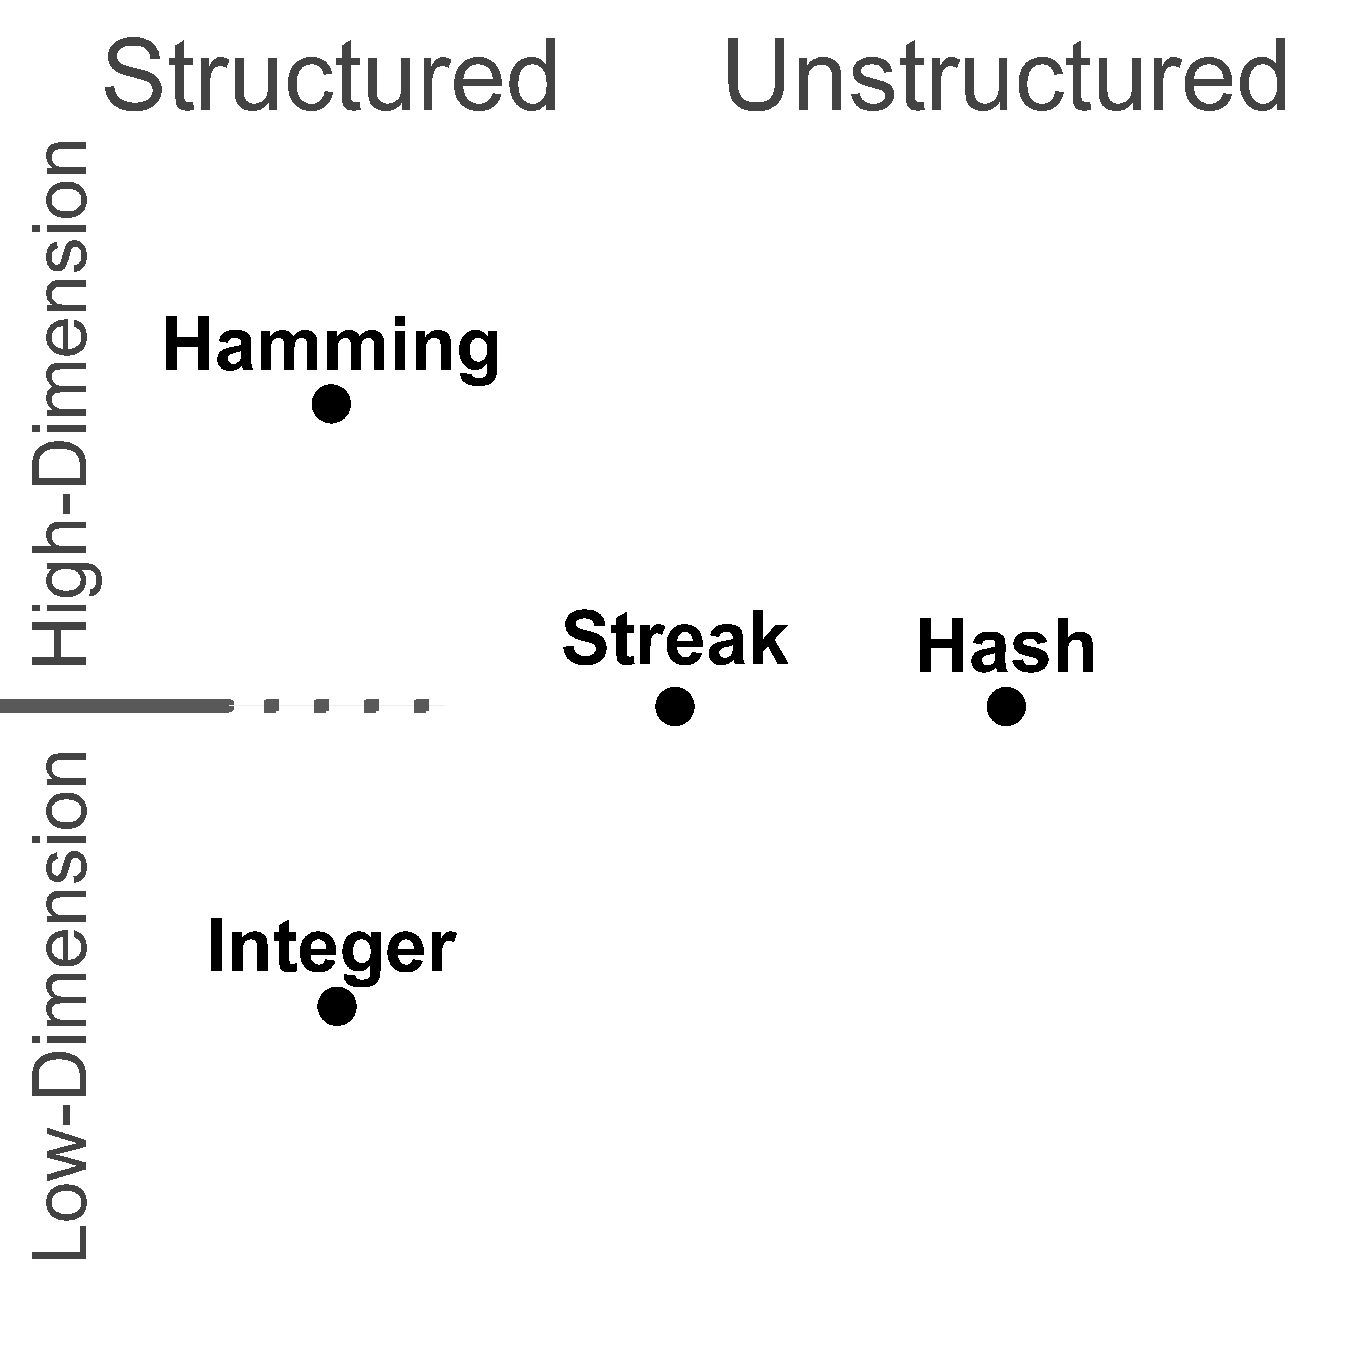
\includegraphics[width=\columnwidth]{img/conceptual-geometry}
\caption{
A conceptual schematic of the tag-matching metrics' geometric properties.
}
\label{fig:conceptual_geometry}

\end{center}
\end{figure}

% First, we performed  %TODO
% If two tags both closely match a third tag, will these two tags be constrained to closely match each other?
% Likewise, if a tag closely matches a second tag, will the tag be constrained to poorly match other tags the second tag poorly matches?

Evolutionary experiments in Section \ref{sec:evolutionary} showed that choice of tag-matching metric had a significant effect on adaptive evolution.
In all experiments, adaptive evolution progressed more slowly under certain metrics than under others.
In most experiments, final solution quality was also affected by tag-matching metric choice.

We found that network constraint (the number of tags a query or operand needs to simultaneously establish affinity with) influenced the relative performance of tag-matching metrics.
% In target-matching evolutionary experiments, network constraint corresponded to degree and regularity of the target graphs.
% In the genetic programming experiments, network constraint corresponded to the interconnectedness of module interaction networks that were selected for.
In target-matching evolutionary experiments, we found that the hash metric enabled rapid adaptive evolution toward targets with low network constraint.
Under high network constraint, however, the hash metric yielded poor-quality solutions.
The integer metrics also yielded poor-quality solutions for target graphs with network constraint.
In some more-constrained cases, the streak metric enabled more rapid adaptive evolution than the Hamming metric.

Geometrical analyses of how tag-matching metrics constrain patterns of connectivity between tags helps to explain the interplay between metrics and problem network constraint.
When problems require tag-matching configurations involving more than a single query-operand tag pair (e.g., a particular query tag matching closely to two different operand tags), these geometric constraints can make certain configurations unlikely or even impossible.
The bidirectional integer metric exhibited the tightest geometrical constraint in our analyses.
The unidirectional integer metric also exhibited tight geometrical constraint, but quirks of its non-commutative construction allowed that constraint to split across perfect- and worst-matching extremes.
Hamming and streak metrics exhibited looser geometric constraint, with the streak metric allowing for edge cases that very strongly break constraints.
Finally, the hash metric exhibited no geometrical constraint because it had no geometrical structure.

Geometrical constraint explains with poor performance of the integer metrics on problems with high network constraint.
However, it is surprising that the geometrically unconstrained hash metric performed best on problems with low network constraint and worst on problems with high network constraint  --- the opposite of what may otherwise be expected.
Analysis of metrics' mutational properties provides an explanation.

Analysis of the effect of bitwise mutation on match distance score revealed significant differences metrics.
Under the Hamming metric, all mutations have small effects on match distance score.
In contrast, under the integer metrics, rare mutations can have strong effects on match distance score.
The streak metric also exhibited strong-effect mutations, particularly with respect to coupling loosely-affiliated tags.
The hash metric exhibited the fattest tails of mutational magnitude, with strong-effect mutations occurring frequently.
Interestingly, the hash metric also exhibited sign-outcome frequencies that differed from the other metrics: mutations that decoupled tightly-matching tags and mutations that coupled loosely-matching tags were more frequent compared to other metrics.

The Hamming metric exhibited the greatest robustness to mutation along mutational walks, followed by the streak metric.
The integer metrics, in particular the unidirectional integer metric, exhibited less robustness.
The hash metric, where all one-step mutations scramble match distance, exhibited the least robustness.

The hash metric's volatility under mutation may explain how it facilitates rapid adaptive evolution in unconstrained problem domains: this rapid evolution may be due to the hash metric's ability to rapidly generate variation.
Likewise, the hash metric's poor performance on high-constraint problem domains may also be explained by mutational volatility.
If tags are selected for to simultaneously satisfy two matching requirements (e.g., to match closely to two other tags), it makes sense that adaptive evolution would be stymied if any change to the focal tag necessarily scrambled behavior on \textit{both} requirements.
This would prevent satisfaction of a single tag-matching requirement from being used as a stepping stone towards satisfaction of both.

Results from evolution experiments with a full-fledged genetic programming system suggest that additional mechanisms may influence tag-matching metric performance.

In genetic programming evolutionary experiments, we found that the Hamming and streak metrics yielded successful solutions the most frequently.
On the directional signal task, which tends to require denser (more constrained) interaction networks, we found evidence that the streak metric enabled more rapid adaptive evolution than the Hamming metric.
The hash metric had the next-best performance in SignalGP experiments, yielding more solutions than the integer metrics, which performed comparably poorly.

Although the hash metric performed best in low-constraint target-matching experiments, it was outperformed in low-constraint SignalGP experiments by the streak and Hamming metrics.
Likewise, the integer metrics were outperformed by the streak and Hamming metrics in low-constraint SignalGP experiments even though they had not been in the low-constraint target-matching experiments.

The mechanisms driving degradation of hash and integer metric performance in the GP experiments remain opaque.
The degradation may be due to better streak and Hash support for duplication and differentiation processes within SignalGP lineages, where instruction and module count can grow over time.
However, altering the graph-matching task to emphasize generation of variation and tag differentiation by disallowing initial tag variation did not reproduce degraded hash and integer metric performance.
Another possible causal difference could be fitness landscape ruggedness.
Within the target-matching experiments, the fitness benefit of a particular query-operand match does not depend on other query-operand matches
In the SignalGP experiments, where modules can form arbitrary interweaving call chains, this is likely not the case.
Further experiments are needed to understand the evolutionary dynamics of non-trivial tag-matching systems and the interplay of those dynamics with tag-matching metrics.

%MAM add subsection divider here?
%\subsection{Synthesis of Metric Properties}

\begin{figure}
\begin{center}

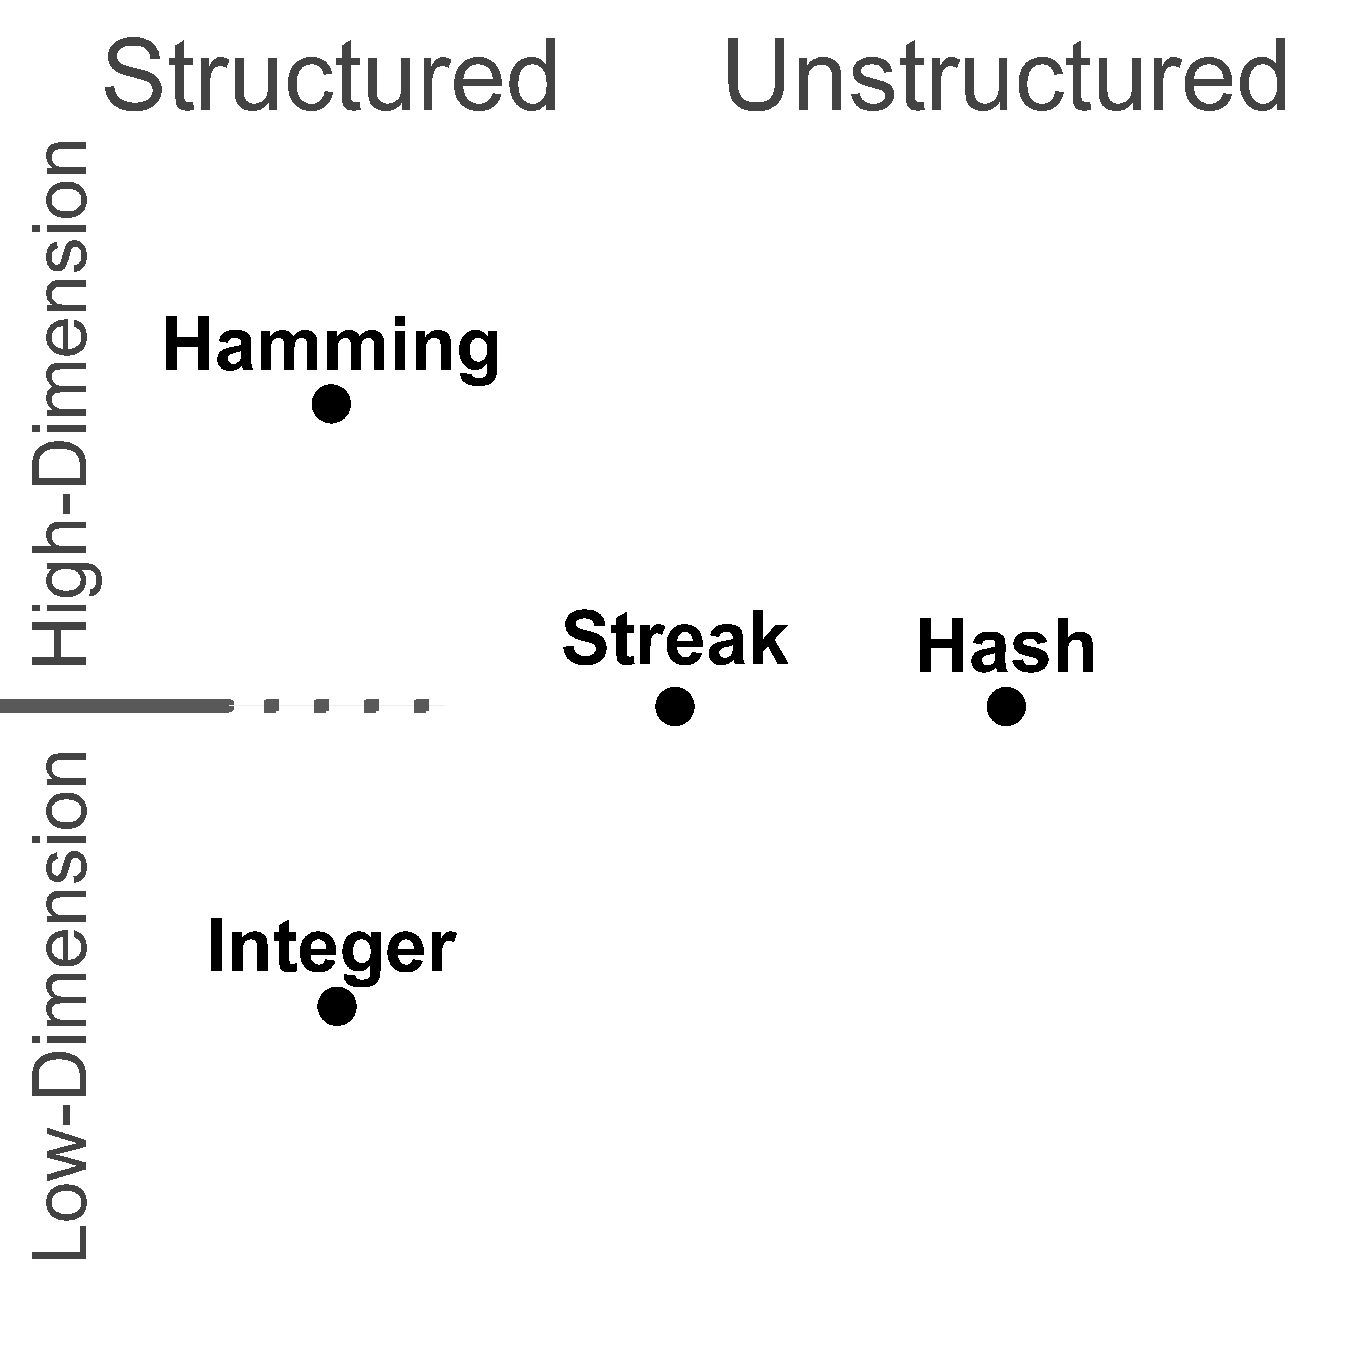
\includegraphics[width=\columnwidth]{img/conceptual-geometry}
\caption{
A conceptual schematic of the tag-matching metrics' geometric properties.
}
\label{fig:conceptual_geometry}

\end{center}
\end{figure}


Relative to the other metrics, the streak metric appears to offer intermediate variational and geometric properties.
Figure \ref{fig:conceptual_geometry} depicts a schematic summary of this observation.
It exhibits some, but not strict, geometric constraint.
Many mutations are neutral or near-neutral (like the integer and Hamming metrics) but a fat tail of extreme-effect mutations also occur (like the hash metric).
The streak metric exhibits robustness under mutational walks that falls between the Hamming and integer metrics.
These mechanistic observations offer a potential explanation for the streak metric's strong performance facilitating adaptive evolution under high-constraint conditions.
However, whether these mechanistic explanations are sufficiently complete --- especially with respect to the streak metric's outperformance of the Hamming metric under high-constraint conditions --- is unclear.

\subsection{Practical Recommendations}

Our results highlight the dependence of tag-matching metrics' performance on problem domain.
So, consideration of properties of the problem domain at hand should drive the decision of which tag-matching metric to use in a particular system.

A major practical advantage of integer-based metrics is the possibility for log time lookup of operands (i.e., via binary search).
However, the integer metrics performed competitively only within a particular class of problem domains.
In all high-constraint problem domains, the integer metrics performed poorly.
Among low-constraint problem domains, the integer metrics only performed well on the toy graph-matching task --- they did not perform well on the low-constraint GP changing signals task.
At present, it is unclear what problem domain property stymied the integer metrics in the low-constraint GP changing signals task --- the potential for the operand set to grow over time (e.g., duplication and divergence), fitness landscape ruggedness (e.g., epistasis), or something else.

However, within the low-constraint target-matching problem domain where integer metrics performed well (i.e., a low-constraint, fixed-size problem with a smooth fitness landscape), the hash metric actually performed slightly better.
So, under these conditions, the hash metric may be preferable when log time lookup is not critical.

Outside the low-constraint target-matching problem domain, the Hamming and streak metrics perform significantly better than the integer metrics.
On the low-constraint target-matching problem, both did evolve full solutions, although the Hamming metric was slightly slower than the streak and integer metrics.
In particular, the Hamming and streak metrics performed best in our GP tests.
So, both metrics appear to be reasonable choices in most cases.

Choosing between the two will likely depend on implementation considerations: the streak metric facilitated faster adaptive evolution in some experiments, but is more computationally expensive to calculate than the Hamming metric.
Future work should investigate whether a streamlined version of the streak metric --- for example, ignoring mismatching streak length and only considering matching streak length --- suffices to capture its properties.

A critical qualification on these recommendations should be noted: they assume the bitwise mutation used in this work.
Although, in supplementary experiments reported in Supplementary Section \ref{sec:graph-matching-norm} we did not find that a simple Gaussian mutation operator improved the performance of integer metrics on the graph-matching task, future work should more thoroughly explore the extent to which our findings generalize under alternate mutation operators.
